% Compile with: lualatex koch_snowflake.tex
\documentclass[11pt]{article}

\usepackage{amsmath, amssymb}
\usepackage{tikz}
\usetikzlibrary{decorations.fractals}
\usepackage[a4paper, margin=2.5cm]{geometry}
\usepackage[colorlinks=true, urlcolor=blue]{hyperref}
\usepackage{fancyhdr}

\pagestyle{fancy}
\fancyhf{}
\renewcommand{\headrulewidth}{0pt}
\fancyfoot[L]{\small Junzhe Wang ~\textperiodcentered~
  \href{mailto:junzhe.wang2002@gmail.com}{\texttt{junzhe.wang2002@gmail.com}}}
\fancyfoot[R]{\small Last edited: \today\ ~\textperiodcentered~ p.\,\thepage}

\title{The Koch Snowflake}
\author{}
\date{}

\begin{document}

\maketitle
\thispagestyle{fancy}

\section{Definition}

The \emph{Koch curve} of depth $n$ between two points $A$ and $B$ is defined
recursively. For $n = 0$ it is simply the segment $[A, B]$. For $n > 0$, the
segment is divided into three equal parts $[A, C]$, $[C, E]$, $[E, B]$, and
the middle part is replaced by the two upper sides of the equilateral
triangle $CED$ erected on it. The curve of depth $n$ then consists of four
Koch curves of depth $n - 1$, along $[A, C]$, $[C, D]$, $[D, E]$ and
$[E, B]$.

\begin{center}
\begin{tikzpicture}[scale=1.1]
  \draw (0, 0) -- (3, 0);
  \node[below] at (0, 0) {$A$};
  \node[below] at (3, 0) {$B$};
  \begin{scope}[xshift=4.5cm]
    \draw (0, 0) -- (1, 0) -- (1.5, {sqrt(3)/2}) -- (2, 0) -- (3, 0);
    \node[below] at (0, 0) {$A$};
    \node[below] at (1, 0) {$C$};
    \node[above] at (1.5, {sqrt(3)/2}) {$D$};
    \node[below] at (2, 0) {$E$};
    \node[below] at (3, 0) {$B$};
  \end{scope}
  \begin{scope}[xshift=9cm, decoration=Koch snowflake]
    \draw decorate { decorate { (0, 0) -- (3, 0) } };
    \node[below] at (0, 0) {$A$};
    \node[below] at (3, 0) {$B$};
  \end{scope}
\end{tikzpicture}

\smallskip
Depths $0$, $1$ and $2$ of the Koch curve.
\end{center}

The \emph{Koch snowflake} is obtained by tracing three Koch curves along the
three sides of an equilateral triangle, bumps pointing outward:

\begin{center}
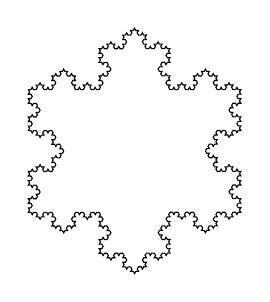
\begin{tikzpicture}[scale=0.9, decoration=Koch snowflake]
  \draw decorate { decorate { decorate { decorate {
    (0, 0) -- (3, 0) -- (1.5, {-3*sqrt(3)/2}) -- (0, 0)
  } } } };
\end{tikzpicture}
\end{center}

\section{The geometry of one step}

With points as vectors, the construction of one step is three formulas:
\begin{equation}
  C = A + \tfrac{1}{3}(B - A), \qquad
  E = A + \tfrac{2}{3}(B - A), \qquad
  D = C + R_{60^\circ}(E - C),
\end{equation}
where $R_{60^\circ}$ is the rotation by $60^\circ$,
\begin{equation}
  R_\theta \begin{pmatrix} x \\ y \end{pmatrix}
  = \begin{pmatrix}
      x \cos\theta - y \sin\theta \\
      x \sin\theta + y \cos\theta
    \end{pmatrix}.
\end{equation}
The sign of the angle decides on which side of $[A, B]$ the bump grows;
flipping it everywhere turns the snowflake into the \emph{anti-snowflake},
whose bumps point inward.

\section{Properties}

Start from an equilateral triangle of side $s$ and area
$A_0 = \frac{\sqrt{3}}{4} s^2$.
\begin{itemize}
  \item \textbf{Exponentially many segments.} Each step replaces one segment
    by four of one third the length: depth $n$ has $4^n$ segments per side,
    each of length $s / 3^n$.
  \item \textbf{Infinite perimeter.} The boundary length is
    $3 s \left(\tfrac{4}{3}\right)^n \to \infty$: the limit curve has
    infinite length, yet fits in a bounded region.
  \item \textbf{Finite area.} Each step adds ever-smaller triangles; the
    total converges to $\tfrac{8}{5} A_0$. An infinite fence around a finite
    lawn.
  \item \textbf{Fractal dimension.} The limit curve is self-similar with
    ratio $3$ producing $4$ copies, so its Hausdorff dimension is
    $\log 4 / \log 3 \approx 1.262$ --- strictly between a line and a plane.
  \item \textbf{Continuous, nowhere differentiable.} The limit curve has a
    corner in every neighborhood of every point; it was one of the early
    ``pathological'' curves (von Koch, 1904).
\end{itemize}

\section{From mathematics to pixels}

The program computes the depth-$n$ curve recursively: a depth-$0$ call
contributes its endpoint, a deeper call delegates to its four children. The
recursion is a \emph{tree} of branching factor four -- unlike a loop-shaped
(tail) recursion, its work grows as $4^n$, which is why the drawing depth is
capped: depth $6$ already traces $3 \cdot 4^6 = 12{,}288$ segments, well
below a pixel each at screen size.

\end{document}
